\chapter{Movement of the Robotic Arm}

\section{Comparison of methods}
There are different ways to perform the mathematical Operations to move a pointobject in a coordinate system. And that's basically what we do here. We have matrices with lots of points in it which built up the modules of our robotic arm and the arm itself.

Four of the possible ways to handle it are explained below together with their advantages and disadvatages.

\subsection{3d Rotation Matrizes and separate Translations}
With this method we have three 3x3 matrices to perform rotational movements. Translational movements needs to be taken care of separately.\\\\
Advantages:\\
- small matrices which doesen't need a lot of cpu power.\\
- easy to use matrices.\\\\
Disadvantages:\\
- Not very clearly arranged\\
- If there are lots alternating rotations and translations it consumes a lot cpu power to calculate all the matrices for all the points. 

\subsection{Principe of Homogen Matrizes}
This method is very similar to the first method. The difference is that you have three 4x4 matrices. This additional dimension allows you to calculate the translation movement the same way as the rotational movement which makes it a lot more intuitive and much faster if you have alternating translation and rotation movements.\\\\
Advantages:\\
- intuitive\\
- fast when calculation many movements for one point\\\\
Disadvantages:\\
- 4x4 matrices which is more calculating work for the computer\\

\subsection{Rodrigues rotation formula}
This is a very easy to use mathematical formula to perform rotations around an allocatable axis. But it only allows rotation movements.\\\\
Advantages:\\
- Very fast\\
- Comprehensive for rotations\\\\
Disatvantages:\\
- Not intuitive because Translational movements must be treated separately\\

\subsection{Quaternions}
Quaternions are an extention of the Gauss number plane created by Sir William Rowan Hamilton. It to allows to perform rotational movements too. But no translations.\\\\
Advantages:\\
- very fast operations\\\\
Disadvantages:\\
- Not intuitive because translations have to be treated seperately.\\
- Quaternions are a pain to calculate\\
- Not supported on matlab, just octave\\

\subsection{Decision}
We decided to build our simulation on the second method (Homogen Matrices) because it's the most intuitive one.

\section{Movement of Arm}
In general one movement persists of at least 5 part movements:\\
- move the object to the world coordinate origin\\
- turn the object to the world coordinate direction\\
- make the movement you want to\\
- turn the object back to the coordinate direction they where befor turning them to the world coordinate directon\\
- move the object to it's original position\\\\
Sometimes we could shorten this general sequence. How we could shorten it will be explained in each case.\\\\
Here's needed to be said, that we never made any sanity checks for movements.\\\\
The following matrices are the one everything builts on:\\\\
Homogeneous Translation Matrix:
\begin{align*}
tl(t_x,t_y,t_z)=
\begin{bmatrix} 
1 & 0 & 0 & t_x \\ 
0 & 1 & 0 & t_y \\ 
0 & 0 & 1 & t_z \\ 
0 & 0 & 0 & 1
\end{bmatrix}
\end{align*}
Homogeneous Rotation Matrix rotation around x-axis:
\begin{align*}
rx(\theta)=
\begin{bmatrix} 
1 & 0 & 0 & 0 \\ 
0 & cos(\theta) & -sin(\theta) & 0 \\ 
0 & sin(\theta) & cos(theta) & 0 \\ 
0 & 0 & 0 & 1
\end{bmatrix}
\end{align*}
Homogeneous Rotation Matrix rotation around y-axis:
\begin{align*}
ry(\theta)=
\begin{bmatrix} 
cos(\theta) & 0 & sin(\theta) & 0 \\ 
0 & 1 & 0 & 0 \\ 
-sin(\theta) & 0 & cos(\theta) & 0 \\ 
0 & 0 & 0 & 1
\end{bmatrix}
\end{align*}
Homogeneous Rotation Matrix rotation around z-axis:
\begin{align*}
rz(\theta)=
\begin{bmatrix} 
cos(\theta) & -sin(\theta) & 0 & 0 \\ 
sin(\theta) & cos(\theta) & 0 & 0 \\ 
0 & 0 & 1 & 0 \\ 
0 & 0 & 0 & 1
\end{bmatrix}
\end{align*}



\subsection{Movement of upper arm}

The upper arm movement is relatively easy because we defined that it's only movement possibilities is up and down. So we just need the homogeneous translation matrix and set $t_x=0$ and $t_y=0$ $t_z=$relative movement.

\subsection{Movement of forearm}
The forearm is a bit more complex, but still not to complex. It's origin isn't the origin of the world coordinate system, so fist step is to move it to the world coordinate system origin.\\
The only movement the forearm can perform is a rotation around the z-axis because of the way it's built up. So next step is to rotate it and after that we can move it back to the starting position.\\\\
$Rot_{matrix}=T(x,y,z)*Rz(\theta)*T(-x,-y,-z)$

\subsection{Movement of hand}
The hand is a general movement as described on top of the chapter.

We name the matrix which turns the roboter coordinate system to the world coordinate system: $rot_{sys}$ (How this matrix is created you can see in the section: Matching coordinate systems)\\
And we name the relativ rotation matrix: $rot_{rel}$ (This is the movment we acually want to perform.)\\
$Rot_{matrix}=T(x,y,z)*inv(rot_{sys})*rot_{rel}*rot_{sys}*T(-x,-y,-z)$

We've written three function with which we can independently rotate around x-axis, y-axis or z-axis. When using them, the user has to make sure to not fall into a Gimbal-Lock(see section Gimbal-Lock).
There are two additional function to perform combined rotations around xyz-axises. One of it with the Gimbal-Lock z-axis direction(turning sequence = zxy), the other with the Gimbal Lock in x-axis direction (turning sequence = xyz).
\subsection{Movement of finger}
The finger movement is very similar to the hand movement, though a bit easier because there is no rotation movement to perform, just a translation movement. This resolves the whole Gimbal-Lock problem. What remains is, that we have to match the coordinate systems because the movement of the hand affects the finger.\\
So the movement matrix looks like:\\
$Move_{matrix}=T(x,y,z)*inv(rot_{sys})*T_{0,0,z}*rot_{sys}*T(-x,-y,-z)$
\pagebreak

\subsection{Matching coordinate systems}
To match two coordinate systems you have to move first the two origins together. Then you've to find the rotation matrix which turns one into the other. That's why we decided that every part of the robotic arm has it's own coordinate system together with a vector which points from the origin of the world coordinate system to the origin of the roboter coordinate system, which is turned and moved together with the corresponding part. This allows us to match the origin easily with just one translation move. The adjusting of the coordinate systems is a bit more tricky. But we know the following thing:\\
Definitions:\\
$e_x$: unit vector in world coordinate x-axis direction\\
$e_y$: unit vector in world coordinate y-axis direction\\
$e_z$: unit vector in world coordinate z-axis direction\\
$e_x'$: unit vector in roboter coordinate x-axis direction\\
$e_x'$: unit vector in roboter coordinate y-axis direction\\
$e_x'$: unit vector in roboter coordinate z-axis direction\\
We know one rotation matrix M must comply with all three rotations. so we get the following three equations:\\
\begin{align*}
M*\vec{e_x}&=\vec{e_x'}\\
M*\vec{e_y}&=\vec{e_y'}\\
M*\vec{e_z}&=\vec{e_z'}\\
\rightarrow 
\begin{bmatrix}
a & b & c\\ d & e & f\\ g & h & i
\end{bmatrix}
\begin{bmatrix}ex_x\\ex_y\\ex_z\end{bmatrix} &= \begin{bmatrix}ex_{x}'\\ex_{y}'\\ex_{z}'\end{bmatrix}\\
\rightarrow 
\begin{bmatrix}
a & b & c\\ d & e & f\\ g & h & i
\end{bmatrix}
\begin{bmatrix}ey_x\\ey_y\\ey_z\end{bmatrix} &= \begin{bmatrix}ey_{x}'\\ey_{y}'\\ey_{z}'\end{bmatrix}\\
\rightarrow 
\begin{bmatrix}
a & b & c\\ d & e & f\\ g & h & i
\end{bmatrix}
\begin{bmatrix}ez_x\\ez_y\\ez_z\end{bmatrix} &= \begin{bmatrix}ez_{x}'\\ez_{y}'\\ez_{z}'\end{bmatrix}\\
\end{align*}  

These are 9 unknown variables and 9 linear equations which can be solved easily with matlab/octave.

\subsection{Calculating Euler Angles}
If we want to scale the the movement of the robotic arm to animate it. we must know the angles to rotate. This angles are called euler angles. Euer angles are always three angles with which we can rotate an object to face any direction we want. The angles depend on the sequence you rotate them. We decide the sequence to be ZYZ.\\

\begin{minipage}{0.5\textwidth}
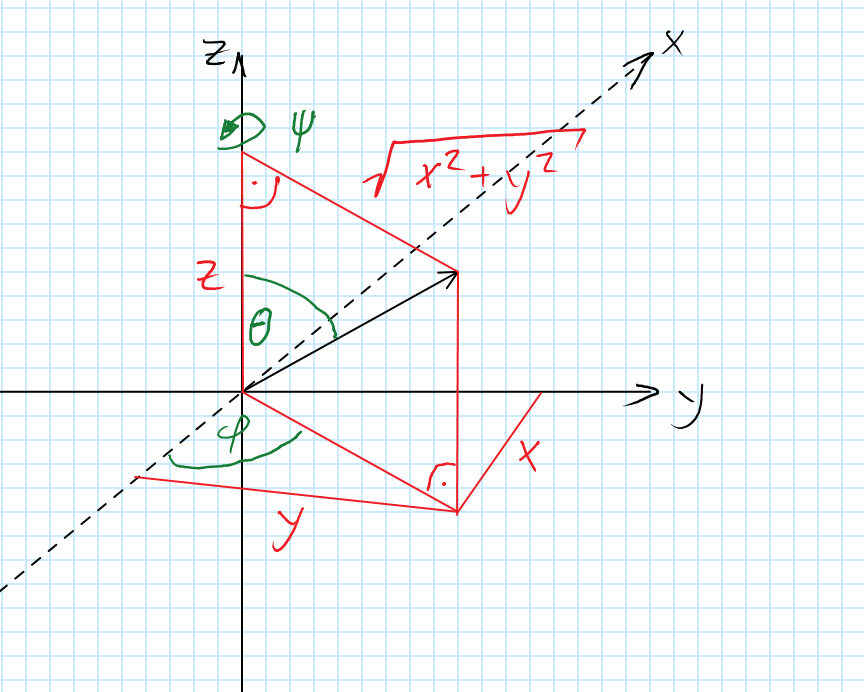
\includegraphics[width=\textwidth]{imgs/AngleCalc/eulerangles.png}
\end{minipage}
\begin{minipage}{0.5\textwidth}
Calculating first two angles from z vector of the coordinate system of the robot:\\
\begin{align*}
\varphi &= arctan(\frac{x}{y})\\
\theta &= arctan(\frac{\sqrt{x^2+y^2}}{z}
\end{align*}
Calculating the last angle:\\
$\rightarrow$ First execute the two rotation, then calculate the last angle from the x-axis or y-axis of the coordinate system. We chose the y-axis:\\
\begin{align*}
\Psi &= arctan(\frac{x}{y})
\end{align*}
\end{minipage}

\subsection{Gimbal-Lock}
Gimbal-Lock is a problem which occurs when rotating an object with euler angles. It occurs because you always have to decide for an order how to rotate the object. For example first rotate around x-axis, then y-axis then z-axis(xyz-order). In this case Gimbal-Lock would occur when the y-axis is 90° to the x-axis and z-axis. It's always the middle axis which is the problem, because it can move the other both in one plane if the first axis isn't moved. The following picture should show it:\\
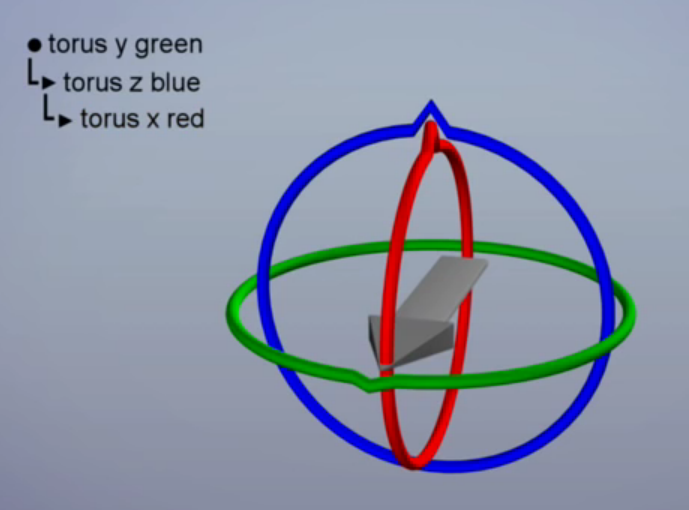
\includegraphics[width=0.45\textwidth]{imgs/GimbalLock/GimbalLock1.png}$\rightarrow$
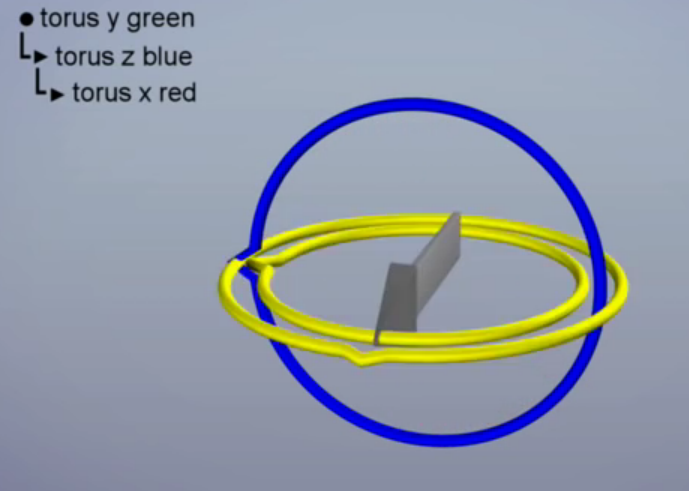
\includegraphics[width=0.45\textwidth]{imgs/GimbalLock/GimbalLock2.png}\\
\textit{(Pictures out of the following you tube video: https://www.youtube.com/watch?v=zc8b2Jo7mno)}

\pagebreak
\subsection{Calculation of rotation angles}
In order to get the arm to move to a certain position, we have to calculate the required angles of rotation of each segment of the arm. We do this with a vector based approach which leads to following system of equations. Alternative approaches would have involved {\em the law of cosins} or {\em complex numbers.} We used vectors due to their simplicity. Following equations are the basis of our calculations:

\begin{align*}
\vec{a}  + \vec{b} = \vec{x}\\
|\vec{a}| = A\\
|\vec{b}| = B
\end{align*}

$\vec{a}$ being the vector representing the upper arm, $\vec{b}$ representing the fore arm, and $\vec{x}$ being the position vector of the destination. $A$ and $B$ are the lengths of each segment. Using the components of the vectors we get following equations:

\begin{align*}
a_x + b_x = x_x\\
a_y + b_y = x_y\\
\sqrt{a_x^2 + a_y^2} = A\\
\sqrt{b_x^2 + b_y^2} = B
\end{align*}

Solving the system for $a_x$, $a_y$, $b_x$, and $b_y$ gives us two sets of components for $\vec{a}$ and $\vec{b}$. The second solution is the same as the first but mirrored along the position vector of the destination. We can therefor just pick a solution.

\begin{center}
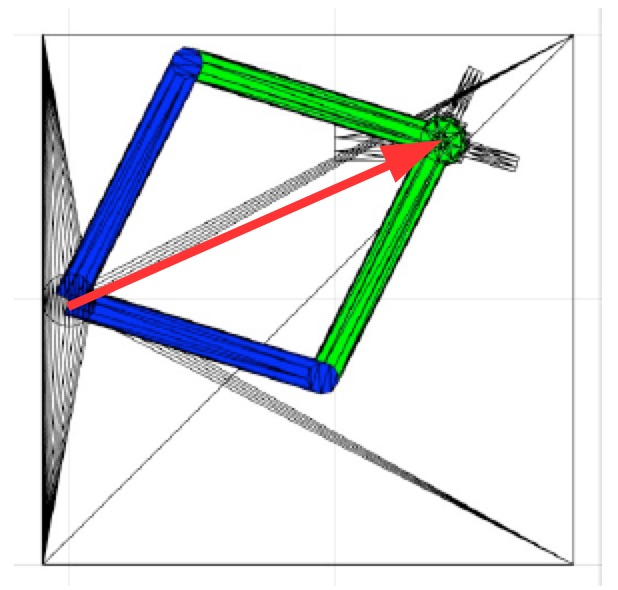
\includegraphics[width=0.45\textwidth]{imgs/AngleCalc/robot_altSolution.jpg}\\
\textit{Showing the the solutions for moving the robot to a given position}
\end{center}

\pagebreak

Calculating the angles of the vectors and considering the rotation of the first segment for the second one, give us the rotation angle of each segment. Subtracting the current angles from the result will give us the relative rotation angle to get from one position to another.

\begin{align*}
\alpha = \arctan(\frac{a_y}{a_x})\\
\beta = \arctan(\frac{b_y}{b_x}) - alpha
\end{align*}

\begin{center}
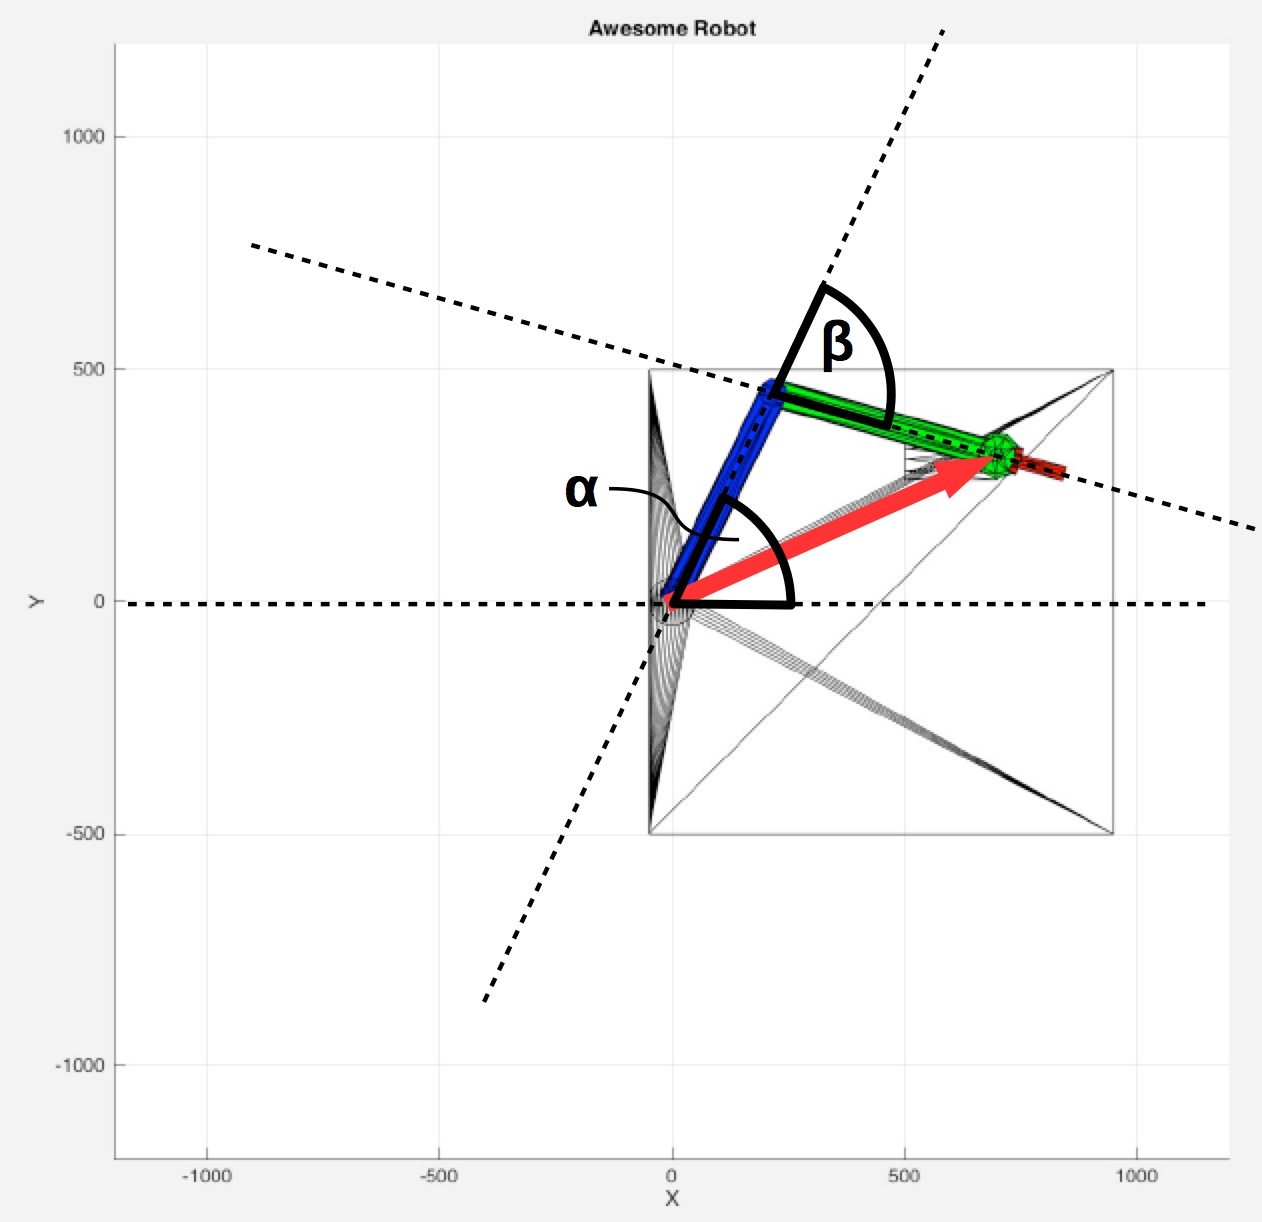
\includegraphics[width=0.45\textwidth]{imgs/AngleCalc/robot_rotAngleCalc.jpg}\\
\textit{Illustration of the problem}
\end{center}

\subsection{Preventing the arm from passing through itself}
A big challange of calculating the rotation angle is to prevent the arm or rather the hand from passing through the pillar. The problem mostly occures when doing more than one rotation. Solving the problem proved to be quite difficult, as we couldn't pedict which of the two solutions we end up with when picking the {\em first.} To eprevent the phenomenon, we can formulate following simple rules:\\

{\em The fore arm must never rotate more than 360 degrees. If the fore arm is left of the upper arm, or has a positive angle, the fore arm should, in general, turn right using a negaive rotation angle and if the fore arm is right of the upper arm, or has a negative angle, the fore arm should, in general, turn left using a positive rotation angle.}

\pagebreak

These rules lead to the fact that the shortes way is not always the correct way. Following graph shows why:

\begin{center}
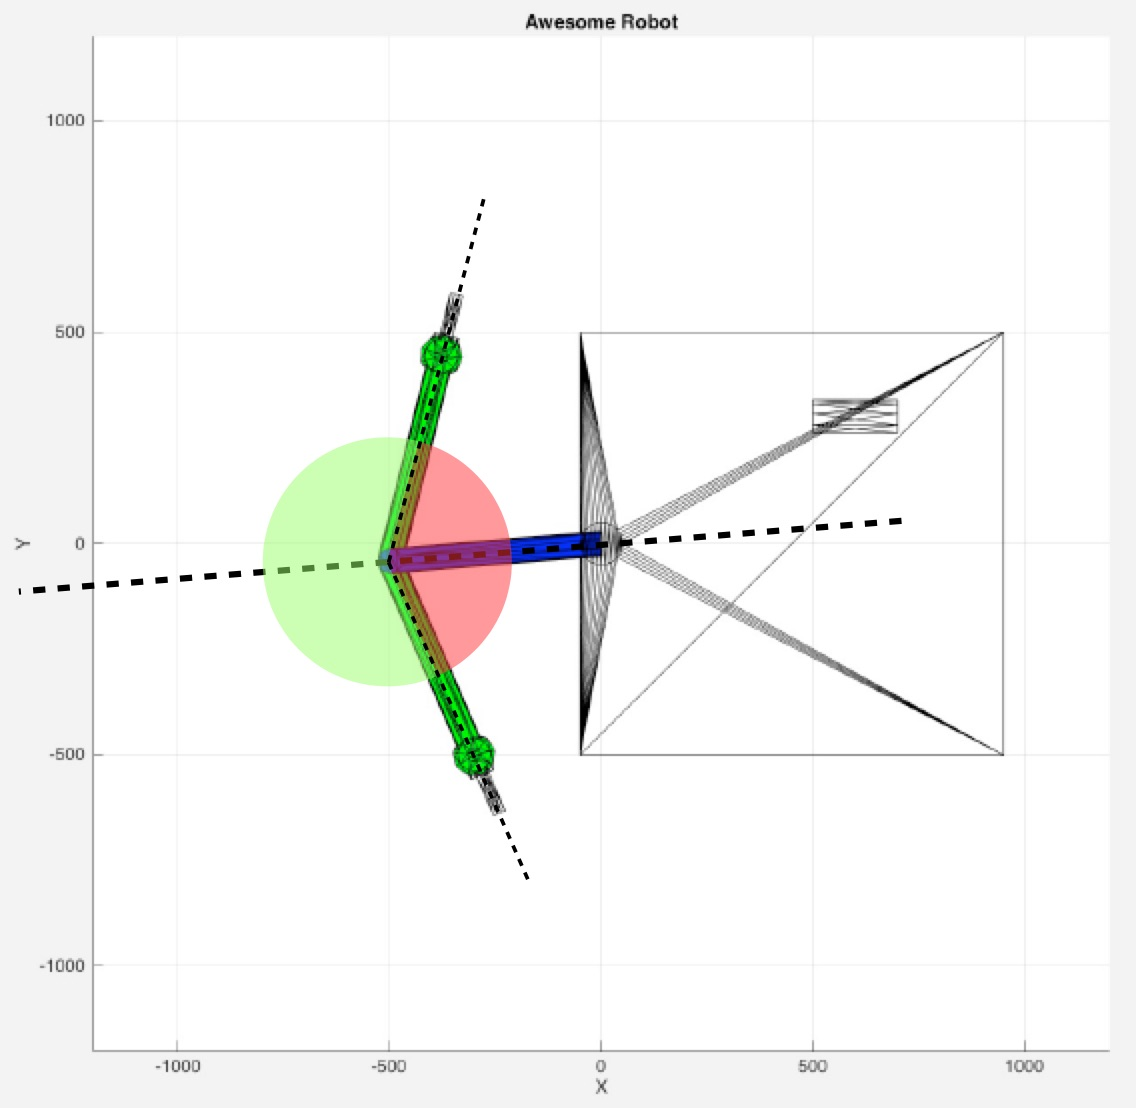
\includegraphics[width=0.45\textwidth]{imgs/AngleCalc/robot_passThroughProblem.jpg}\\
\textit{Red shows the bad rotation angle and green the correct rotation angle}
\end{center}

Following code in {\em MatLab} does the trick:

\begin{framed}\begin{verbatim}
dest_angles = calcArmAngles(dest_pos, robo.upperArm_len, robo.foreArm_len, robo.hand_len);
angles = dest_angles - robo.pos_angles;
    
% making sure that the arm does not pass through itself
angles = rem(angles, 360);
if robo.pos_angles(2) <= 0
        if angles(2) > 0 & abs(angles(2)) > abs(180 - robo.pos_angles(2))
                angles(2) = angles(2) - 360;
        elseif angles(2) < 0 & abs(angles(2)) > abs(180 + robo.pos_angles(2))
                angles(2) = angles(2) + 360;
        end
elseif robo.pos_angles(2) > 0
        if angles(2) > 0 & abs(angles(2)) > abs(180 - robo.pos_angles(2))
                angles(2) = 360 - angles(2);
        elseif angles(2) < 0 & abs(angles(2)) > abs(180 + robo.pos_angles(2))
                angles(2) = angles(2) + 360;
        end
end
\end{verbatim}\end{framed}

At first we calculate the relative rotation angles to get to the destination. We then make sure that we don't turn more than 360 degrees by calculating the remainder {\em 'rem'} from a division with 360. We then basically apply the rule above: if the fore arm is to the left, turn right and if the fore arm is to the right, turn left. But of course, we also allow small rotations to the left if the fore arm is to the left and the other way around. But all under the restriction that the fore arm never turns more than {\em 180 degrees plus his current rotation} or {\em 180 degrees minus his current rotation}, depending on his position and the destination. This prevents the hand from passing through the pillar.

